
\begin{document}

\frame{\titlepage}

\begin{frame}{Mathematics textbook conversion}

No reliable, fast, and inexpensive way of producing Braille versions of mathematics texts.

Several tools will produce convincing-looking, but incorrect output.
\pause

Approach implemented by Rob Beezer:
\begin{itemize}
\item
Use PreTeXt for document structure (XML vocabulary that uses \LaTeX\ for mathematics expressions);
\item
Use Liblouis for literary text and the document structure;
\item
Use Speech Rule Engine for mathematics.
\end{itemize}

\end{frame}


\begin{frame}{Graphics conversion}

Starting point: TiKZ diagram, with some preparation. All the coordinates for node locations with labels need to be explicitly defined.

\begin{itemize}
\item
The labels are processed by Liblouis/SRE;
\item
Braille labels are measured, boxes for them are made;
\item
The entire image is measured and scaled as much as possible to fit onto a page;
\item
Temporary SVG file is produced with {\tt dvisvgm};
\item
In SVG, the boxes are replaced with Braille text of the label.
\end{itemize}

\end{frame}


\begin{frame}{Example}

\centering

\begin{tikzpicture}[scale=0.4]

\draw [->]  (0,-5) -- (0,5);
\draw  [->] (-8,0) -- (8,0);
\node [right] at (0,5) {$y$};
\node [below] at (8,0) {$x$};
\node [below] at (0.5,0) {$0$};

\draw (0,0) -- (35:6);
\draw (2,0) arc (0:35:2);

\filldraw[fill=black, draw=black] (35:6) circle (0.05cm);
\node [right] at (35:6) {$a + bi$};
\node [above] at (35:3) {$r$};
\node [right] at (17:2) {$\theta$};
%\node[above] at (current bounding box.north) {Polar coordinates of a complex number};
\end{tikzpicture}


\end{frame}

\begin{frame}{Example}

\centering
\includegraphics{cyclic-complex-polar_svg.pdf}
\end{frame}


\begin{frame}{Example}

\centering
\includegraphics{cyclic-complex-polar.pdf}
\end{frame}


\begin{frame}{Tactile graphics: the last yard}
\protect\hypertarget{tactile-graphics-the-last-yard}{}
Difficulties with tactile graphics do not end after an electronic image
with Braille is created. 


\begin{figure}
\centering
\includegraphics{Embosser.jpg}
\caption{ViewPlus embosser}
\end{figure}
\end{frame}

\begin{frame}{Example}

\begin{figure}
\centering
\includegraphics{finite-field-subfields-sighted.pdf}
\end{figure}

\end{frame}

\begin{frame}
The result is 

\begin{figure}
\centering
\fbox{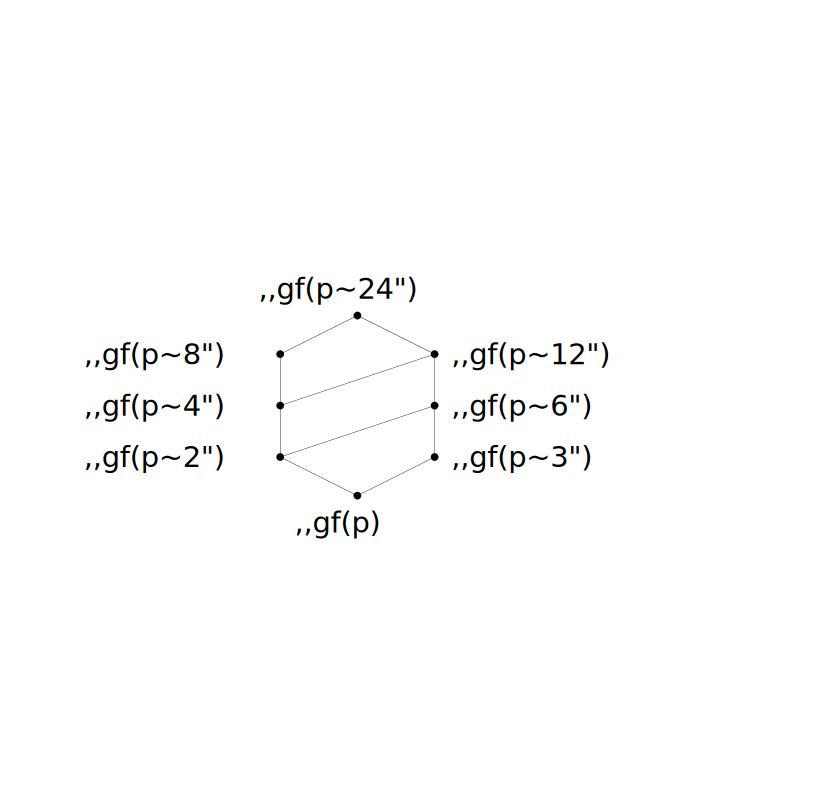
\includegraphics{finite-field-subfields-tactile.pdf}}
\end{figure}

\end{frame}


\begin{frame}
And this is the hard copy:

\begin{figure}
\centering
\includegraphics{diagram_bad.jpg}
\end{figure}
\end{frame}

\begin{frame}
After some settings

\begin{figure}
\centering
\includegraphics{diagram_better.jpg}
\end{figure}

\end{frame}



\begin{frame}
After converting to PDF and un-embedding fonts:

\begin{figure}
\centering
\includegraphics{diagram_best.jpg}
\end{figure}

\end{frame}

\begin{frame}{Points}


\begin{itemize}
\item
Braille needs to be checked for correctness


\vfill

\item
Good-looking image on the screen frequently does not look good embossed

\vfill

\item
Internal structure of the file matters

\vfill
\item
Embedding fonts (or labels) is bad for Braille

\end{itemize}

\vfill
\vfill


\end{frame}



\end{document}
